\documentclass[../main.tex]{subfiles}

\begin{document}
	%http://tex.stackexchange.com/questions/230149/label-a-word-or-sentence
	\makeatletter
	\newcommand{\setword}[2]{%
		\phantomsection
		#1\def\@currentlabel{\unexpanded{#1}}\label{#2}%
	}
	\makeatother
	
	\section{Raggiungibilit\'a e controllabilit\'a}
		Dato un sistema $ \dot x = A x + B u $:\\
		
		$ \hat x $ \'e uno stato \textbf{raggiungibile} in un tempo $ \hat t $ se $ \exists \hat u(t)\ con\ t \in [0, \hat t] $ tale che se $ x(0^-) = 0 $ e $ u(t) = \hat u(t) $, allora $ x(\hat t) = \hat x $.
		\[ X_R(\hat t)\ \text{sottospazio degli stati raggiungibili in}\ \hat t \]
		
		$ \tilde x $ \'e uno stato \textbf{controllabile} in un tempo $ \tilde t $ se $ \exists \tilde u(t)\ con\ t \in [0, \tilde t] $ tale che se $ x(0^-) = \tilde x $ e $ u(t) = \tilde u(t) $, allora $ x(\tilde t) = 0 $.
		\[ X_C(\hat t)\ \text{sottospazio degli stati controllabili in}\ \hat t \]
		
	\subsection{Propriet\'a per i sistemi LTI a tempo continuo}
		Per i sistemi LTI a tempo continuo valgono le seguenti propriet\'a:
		\begin{itemize}
			\item
				se $ \tilde x $ \'e raggiungibile in $ \tilde t $, se e solo se $ \tilde x $ \'e controllabile.
				\[ X_R(\tilde t) \equiv X_C(\tilde t) \]
				Questo \'e dovuto all'invertibilit\'a della matrice $ e^{A \tilde t} $ (che per la propriet\'a dell'esponenziale si pu\'o calcolare come $ \left( e^{A \tilde t} \right)^{-1} = e^{-A \tilde t} $).
				
			\item
				se $ \tilde x \in X_R(\tilde t) $, allora $ \tilde x \in X_R(\hat t) \forall \hat t > 0 $.
				Lo stesso vale per $ X_C $ per la propriet\'a precedente.
				
				Per i SLTI si parla dunque di $ X_R \equiv X_C $ indipendentemente dal tempo.\\
				Prendiamo:
				\begin{itemize}
					\item
						$ \dot x = A x + B u $ \'e un sistema completamente controllabile in $ \tilde t $;
					\item
						dato uno stato iniziale $ x(0^-) = \hat x $, voglio ottenere che lo stato in $ \tilde t $ sia: $ x(\tilde t) = \tilde x $;
				\end{itemize}
				Dimostriamo questa propriet\'a per un determinato controllo:
				\[ \tilde u(\tau) = B^T e^{A^T (\tilde t - \tau)} \cdot \left[ \int_{0^-}^{\tilde t} e^{A(\tilde t - \epsilon)} B B^T e^{A^T (\tilde t - \epsilon)} d\epsilon \right]^{-1} \cdot \left( \tilde x - e^{A \tilde t} \hat x \right) = B^T e^{A^T (\tilde t - \tau)} \cdot W^{-1}(\tilde t) \cdot \left( \tilde x - e^{A \tilde t} \hat x \right) \]
				Applico l'equazione di Lagrange per calcolare $ x(\tilde t) $:
				\begin{align*}
					x(\tilde t) &= e^{A \tilde t} \hat x + \underbrace{\int_{0^-}^{\tilde t} e^{A(\tilde t - \tau)} B B^T e^{A^T (\tilde t - \tau)}}_{W(\tilde t)} W^{-1}(\tilde t) \left( \tilde x - e^{A \tilde t} \hat x \right) =\\
					&= e^ {A \tilde t} \hat x + \left[ W(\tilde t) W^{-1}(\tilde t) \right] \left( \tilde x - e^{A \tilde t} \hat x \right) = \hat x \quad \forall \tilde t > 0
				\end{align*}
				Ho dimostrato che partendo da dove voglio $ \hat x $, arrivo dove voglio $ \tilde x $ in un tempo a piacere, se prendo il giusto controllo $ \tilde u(t) $.
		\end{itemize}
	
		Inoltre valgono le seguenti propriet\'a per $ X_R \equiv X_C $:
		\begin{itemize}
			\item
				$ X_R $ \'e invariante rispetto ad A:
				\[ \tilde x \in X_R \quad\Rightarrow\quad A \tilde x \in X_R \]
				cio\'e se \'e controllabile, allora posso imporre la direzione con cui lo stato si muove.
			\item
				$ X_R $ \'e invariante per il sistema:
				\[ x(\hat t) \in X_R \quad\Rightarrow\quad x(t) \in X_R \forall t \geq \hat t \]
				cio\'e se lo stato \'e dentro lo spazio di raggiungibilit\'a, ci rimane per sempre.
			\item
				$ X_R $ \'e un sottospazio lineare: se posso raggiungere due stati $ \tilde x_1 $ e $ \tilde x_2 $, allora posso raggiungere una qualunque combinazione lineare.\\
				Possiamo dimostrarlo con la propriet\'a di sovrapposizione degli effetti:
				dati $ x_A, x_B \in X_R $
				\begin{itemize}
					\item $ x(0^-) = 0 \Rightarrow \exists u_A(\tau) \Rightarrow x(\hat t) = x_A $
					\item $ x(0^-) = 0 \Rightarrow \exists u_B(\tau) \Rightarrow x(\hat t) = x_B $
				\end{itemize}
				\[ u(\tau) = \alpha u_A(\tau) + \beta u_B(\tau) \Rightarrow x(\hat t) = \alpha x_A + \beta x_B \]
				
				Poich\'e si tratta di un sottospazio lineare, $ \tilde x = 0 $ \'e sempre incluso in $ X_R $. Quindi non esiste un sistema con $ X_R $ insieme vuoto, perch\'e l'origine c'\'e sempre.
		\end{itemize}
		
	\subsection{Completa controllabilit\'a}
		Supponiamo di avere il seguente sistema:
		\[
			\begin{bmatrix}
				\dot{\underline x_1} \\ \dot{\underline x_2}
			\end{bmatrix} = 
			\begin{bmatrix}
				A_{11} & A_{12}\\
				0 & A_{22}
			\end{bmatrix}
			\begin{bmatrix}
				\underline x_1 \\ \underline x_2
			\end{bmatrix} +
			\begin{bmatrix}
				B_1 \\ 0
			\end{bmatrix} \underline u(t)
		\]
		Dalla seconda equazione vedo che $ \underline x_2 $ da $ \underline u $ direttamente n\'e indirettamente attraverso $ \underline x_1 $. $ \underline x_2 $ non \'e controllabile e quindi il sistema non \'e \textbf{completamente controllabile}.
	
	\subsubsection*{Esempio}
		\[
			\underline{\dot x} =
			\begin{tikzpicture}[baseline=-0.5ex]
			\matrix [matrix of math nodes,left delimiter={[},right delimiter={]}] (m)
			{
				0 & 1 & 1 & 0\\
				0 & 0 & 0 & 19\\
				0 & 0 & 0 & 1\\
				0 & 0 & -1 & 0\\
			};  
			\draw[color=red] (m-3-1.north west) -- (m-3-2.north east) -- (m-4-2.south east) -- (m-4-1.south west) -- (m-3-1.north west);
			\end{tikzpicture} \underline x +
			\begin{tikzpicture}[baseline=-0.5ex]
			\matrix [matrix of math nodes,left delimiter={[},right delimiter={]}] (m)
			{
				0\\
				1\\
				0\\
				0\\
			};  
			\draw[color=red] (m-3-1.north west) -- (m-3-1.north east) -- (m-4-1.south east) -- (m-4-1.south west) -- (m-3-1.north west);
			\end{tikzpicture} \underline u
		\]
		Si nota che la seconda componente dello stato non \'e controllabile:
		\[
			\underline{\dot x_2} =
			\begin{bmatrix}
				0 & 1\\
				-1 & 0
			\end{bmatrix} \underline{x_2}
		\]
		Quindi il sistema non \'e completamente controllabile.\\
		Per esercizio calcoliamo la trasformata della soluzione di questa equazione differenziale:
		\[
			X_2(s) =
			\begin{bmatrix}
				s & -1\\
				1 & s
			\end{bmatrix}^{-1} \underline x(0^-) =
			\begin{bmatrix}
				\frac{s}{s^2+1} & \frac{1}{s^2+1}\\
				\frac{-1}{s^2+1} & \frac{s}{s^2+1}
			\end{bmatrix} \underline x(0^-) =
		\]
		Antitrasformiamo:
		\[
			\underline x_2(t) =
			\begin{bmatrix}
				\cos t & \sin t\\
				-\sin t & \cos t
			\end{bmatrix} 1(t) \underline x(0^-)
		\]
		
	\subsection{Teorema di Cayley-Hamilton}
		Data una matrice quadrata $ A \in \R^{n_x \times n_x} $ e il relativo polinomio caratteristico $ \phi(s) = det(sI-A) $, allora:
		\[ \phi(A) = 0\ \text{matrice nulla} \]
		In generale:
		\[ \phi(s) = s^{n_x} + \phi_{n_x-1} s^{n_x-1} + \dots + \phi_1 s + \phi_0 \]
		Per il teorema di Cayley-Hamilton:
		\begin{align}
			\label{th_ch}
			\phi(A) &= A^{n_x} + \phi_{n_x-1} A^{n_x-1} + \dots + \phi_1 A + \phi_0 I = 0\\
			A^{n_x} &= -\phi_{n_x-1} A^{n_x-1} - \dots - \phi_1 A - \phi_0 I
		\end{align}
		$ A_{n_x} $ \'e combinazione lineare di $ I, A, \dots, A_{n_x-1} $.
		
	\subsubsection{Come calcolare $ A^{n_x+k} \forall k \geq 0 $}
		Per esempio cominciamo da $ k = 1 $:
		\[ A^{n_x+1} = A^{n_x} A = \underbrace{- \phi_{n_x-1} A^{n_x}}_{\text{comb. lineare di}\ I, A, \dots, A_{n_x-1}} \underbrace{- \phi_{n_x-2} A^{n_x-1} - \dots - \phi_1 A^2 - \phi_0 A}_{\text{comb. lineare di}\ I, A, \dots, A_{n_x-1}} \]
		Quindi $ A^{n_x+1} $ \'e combinazione lineare di $ I, A, \dots, A_{n_x-1} $.\\
		In generale $ A^{n_x+k} $ \'e combinazione lineare di $ I, A, \dots, A_{n_x-1} $.
		
	\subsubsection{Com'\'e fatto $ X_R $}
		se ipotizziamo $ \underline x(0^-) $:
		\[ X_R = \left\lbrace \text{sottospazio di tutti i}\ \tilde x\ \text{raggiungibili} \right\rbrace = \left\lbrace \int_{0^-}^{\tilde t} e^{A(\tilde t - \tau)} B \tilde u(\tau) d\tau, \forall \tilde t \right\rbrace \]
		L'integrale pu\'o essere visto come combinazione lineare di infiniti termini tra $ e^{A(\tilde t - \tau)} B $ e $ u(\tau) $:
		\[ X_R = \left\lbrace \text{tutte le possibili combinazioni lineari di tutte le colonne di}\ e^{A(\tilde t - \tau)} B \right\rbrace \]
		Ma abbiamo visto che $ e^{At} = \sum_{k=0}^{\infty} \dfrac{A^k t^k}{k!} $:
		\begin{align*}
			e^{A(\tilde t - \tau)} &= \sum_{k=0}^{\infty} \dfrac{A^k (\tilde t - \tau)^k}{k!} = \sum_{k=0}^{\infty} \dfrac{(\tilde t - \tau)^k}{k!} A^k =\\
			&= I + \alpha_1 A^1 + \alpha_2 A^2 + \dots + \alpha_{n_x-1} A^{n_x-1} + \sum_{k=n_x}^{\infty} \alpha_k A^k
		\end{align*}		
		Abbiamo dimostrato che $ A^k $ \'e combinazione lineare di tutti i termini precedenti $ I, A, \dots, A_{n_x-1} $. Quindi:
		\[ e^{A(\tilde t - \tau)} = \text{combinazione lineare}(I, A, \dots, A_{n_x-1}) \]
		In definitiva l'integrale \'e combinazione lineare delle colonne di $ e^{A(\tilde t - \tau)} B \forall (\tilde t - \tau) $, che equivale a una matrice del tipo:
		\[ \left[ B | AB | \dots | A^{n_x-1} B \right] \]

	\subsection{Teorema di Kalmann di raggiungibilit\'a}
		$ X_R $ \'e combinazione lineare di tutte le colonne di:
		\[ P = \left[ B | AB | \dots | A^{n_x-1} B \right] \]
		Il teorema si pu\'o anche scrivere come:
		\[ X_R = Immagine\left( \left[ B | AB | \dots | A^{n_x-1} B \right] \right) \]
		
	\subsubsection*{Esempio}
		Alcune volte non tutte le colonne di $ P $ sono necessarie:
		\[
			\underline{\dot x} =
			\begin{bmatrix}
				0 & 1\\
				10 & 5
			\end{bmatrix} \underline x +
			\begin{bmatrix}
				1 & 1\\
				0 & 1
			\end{bmatrix} \underline u
		\]
		Ci sono 2 variabili di controllo $ n_u = 2 $ e 2 variabili di stato $ n_x = 2 $.
		\[
			P = \left[ B | AB \right] =
			\begin{bmatrix}
				1 & 1 & | & \dots\\
				0 & 1 & | & \dots
			\end{bmatrix}
		 \]
		 In questo caso solo con $ B $ ho gi\'a $ n_x = 2 $ colonne linearmente indipendenti: $ \begin{smallmatrix}1\\ 0\end{smallmatrix} $ e $ \begin{smallmatrix}1\\ 1\end{smallmatrix} $. Quindi \'e inutile scrivere le matrici successive di $ P $, perch\'e le loro colonne saranno sicuramente linearmente dipendenti a quelle di $ B $.
		 
		 In conclusione $ dim\left( X_R \right) = 2 $.
		 
	\subsection{Corollari del teorema di Kalmann}
		\begin{itemize}
			\item 
				\[ dim\left( X_R \right) = rank\left( P \right) \]
				La matrice $ P $ ha un numero di colonne e righe pari a:
				\[ P = \left. \left[ \underbrace{\underbrace{B}_{n_u} | \underbrace{AB}_{n_u} | \dots | \underbrace{A^{n_x-1} B}_{n_u}}_{n_u \times n_u \text{colonne}} \right] \right\rbrace\text{$ n_x $ righe} \]
				Quindi il rango di $ P $ pu\'o essere al massimo $ n_x $.
			\item 
				\[ X_R \equiv \R^{n_x} \quad\Leftrightarrow\quad rank\left( P \right) = n_x \quad\Leftrightarrow\quad \text{sistema completamente controllabile} \]
			\item 
				\[ rank\left( P \right) + dim\left( ker\left( P \right) \right) = n_x \]
				dove $ ker $ \'e l'operatore kernel: $ ker\left( P \right) = \underline v | P \underline v = 0 $
			\item 
				Il teorema di Kalmann di raggiungibilit\'a pu\'o essere applicato separatamente su ogni singola variabile di controllo o gruppi di esse.
		\end{itemize}
	
	\subsubsection*{Esempio}
		In questo sistema non tutti i controlli sono necessari per controllare il sistema.
		\[
			\underline{\dot x} =
			\begin{bmatrix}
				0 & 1\\
				0 & 0
			\end{bmatrix} \underline x +
			\begin{bmatrix}
			1 & 0\\
			0 & 1
			\end{bmatrix} \underline u 
		\]
		\[
			P =
			\begin{bmatrix}
				1 & 0 & | & 0 & 1\\
				0 & 1 & | & 0 & 2
			\end{bmatrix}
		\]
		$ rank\left( P \right) = n_x = 2 $ quindi il sistema \'e completamente controllabile se usiamo entrambi i controlli.
		
		Adesso proviamo ad usare solo $ u_1 $:
		\[
			P_1  = \left[ B_1 | AB_1 \right] =
			\begin{bmatrix}
				1 & | & 0\\
				0 & | & 0
			\end{bmatrix}
		\]
		$ rank\left( P_1 \right) \neq 2 $ quindi il sistema non \'e completamente controllabile con $ u_1 $.
		
		Applichiamo solo $ u_2 $:
		\[
		P_2  = \left[ B_2 | AB_2 \right] =
			\begin{bmatrix}
				0 & | & 1\\
				1 & | & 0
			\end{bmatrix}
		\]
		$ rank\left( P_2 \right) = 2 $ quindi il sistema \'e completamente controllabile con $ u_2 $.
		
	\subsection{Cambio di base}
		Prendiamo una matrice quadrata e invertibile $ T $. Il cambio di base sar\'a descritto dalla relazione:
		\[ x = Tz \]
		
		Effettuiamo il cambio di base:
		\begin{align*}
			\dot z &= \dot{(Tz)} = T \dot z = ATz + Bu\\
			y &= CTz + Du
		\end{align*}
		Moltiplichiamo la prima equazione a sinistra per $ T^{-1} $:
		\begin{align}
			\dot z &= T^{-1}ATz + T^{-1}Bu = \tilde A z + \tilde B u\\
			y &= CTz + Du = \tilde C z + \tilde D u
		\end{align}
		
		La funzione di trasferimento non cambia perch\'e il cambiamento di base coinvolge solo lo stato del sistema, non la relazione ingresso uscita:
		\[ T(s) = C(sI-A)^{-1}B+D = \tilde C (sI-\tilde A)^{-1} \tilde B + \tilde D \]
		
		Si pu\'o verificare attraverso il teorema di Kalmann che lo spazio di raggiungibilit\'a \'e invariante rispetto al cambio di base:
		\[ Z_R = Im\left\lbrace \tilde P = \left[ \tilde B | \tilde A \tilde B | \dots | \tilde A^{n_x-1} \tilde B \right] \right\rbrace \]
		\begin{align*}
			\tilde B &= T^{-1} B\\
			\tilde A \tilde B &= T^{-1}AT T^{-1}B = T^{-1}AB\\
			\vdots\\
			\tilde A^{n_x-1} \tilde B &= T^{-1}A^{n_x-1}B
		\end{align*}
		Quindi:
		\[ \tilde P = \left[ T^{-1} B | T^{-1} AB | \dots | T^{-1} A^{n_x-1}B \right] = T^{-1} \left[ B | AB | \dots | A^{n_x-1}B \right] = T^{-1}P \]
		Il sottospazio degli stati raggiungibili nella nuova base \'e:
		\[ Z_R = T^{-1} X_R \]
		
		\begin{Exercise}[title={Studiare la controllabilit\'a di due rami RC in parallelo}, difficulty=3]
			\begin{center}
				\begin{circuitikz} \draw
					(0,0)	to[V, v=u] (0,6)
							to[short](4,6)
							to[short](8,6)
					(4,6)	to[short, i=$ i_1 $](4,5)
							to[R, l=$ R_1 $](4, 3)
							to[C, l=$ C_1 $, v<=$ v_1 $](4,0)
					(8,6)	to[short, i=$ i_2 $](8,5)
							to[R, l=$ R_2 $](8, 3)
							to[C, l=$ C_2 $, v<=$ v_2 $](8,0)
							to[short](0,0)
					;
				\end{circuitikz}
			\end{center}

			Nei circuiti a parametri concentrati, le variabili di stato possono essere identificate con i dispositivi che accumulano energia (in questo caso i condensatori):
			\[ x_1 \triangleq v_1 \qquad x_2 \triangleq v_2 \]
			
			Scriviamo le equazioni delle maglie:
			\begin{align*}
				u &= R_1 i_1 + v_1 \quad\Rightarrow i_1 = \dfrac{1}{R_1} (u-v_1)\\
				u &= R_2 i_2 + v_2 \quad\Rightarrow i_2 = \dfrac{1}{R_2} (u-v_2)
			\end{align*}
			Le sostituiamo nelle equazioni descrittive dei condensatori:
			\begin{align*}
				\dot v_1 &= \dfrac{1}{C_1} i_1 = \dfrac{1}{R_1 C_1} (u-v_1)\\
				\dot v_2 &= \dfrac{1}{C_2} i_2 = \dfrac{1}{R_2 C_2} (u-v_2)
			\end{align*}
			
			Ridefiniamo le costanti di tempo:
			\[ \dfrac{1}{R_1 C_1} = \dfrac{1}{\tau_1} \triangleq \alpha_1 \qquad \dfrac{1}{R_2 C_2} = \dfrac{1}{\tau_2} \triangleq \alpha_2 \]
			dove $ \alpha_1 \neq 0 $ e $ \alpha_2 \neq 0 $.
			
			Le equazioni di stato del sistema diventano:
			\[
				\begin{cases}
					\dot x_1 &= -\alpha_1 x_1 + \alpha_1 u\\
					\dot x_2 &= -\alpha_2 x_2 + \alpha_2 u
				\end{cases}
				\qquad
				\dot x =
				\begin{bmatrix}
					-\alpha_1 & 0\\
					0 & -\alpha_2
				\end{bmatrix} x+
				\begin{bmatrix}
					\alpha_1\\
					\alpha_2
				\end{bmatrix} u
			\]
			
			Calcoliamo la matrice $ P $:
			\[
			P =
			\begin{bmatrix}
				\alpha_1 & | & -\alpha_1^2\\
				\alpha_2 & | & -\alpha_2^2
			\end{bmatrix}
			\]
			\[ det(P) = -\alpha_1 \alpha_2^2 + \alpha_1^2 \alpha_2 = -\alpha_1 \alpha_2(\alpha_2-\alpha_1) \]
			\[ det(P) \neq 0 \Leftrightarrow \alpha_1 \neq \alpha_2 \Leftrightarrow X_R = \R^2 \]
			il sistema \'e completamente raggiungibile.
			
			Nel circuito equivale a $ \tau_1 \neq \tau_2 \Leftrightarrow R_1 C_1 \neq R_2 C_2 $.
			\begin{figure}[h!]
				\centering
				\resizebox{.7\columnwidth}{!}{% GNUPLOT: LaTeX picture with Postscript
\begingroup
  \makeatletter
  \providecommand\color[2][]{%
    \GenericError{(gnuplot) \space\space\space\@spaces}{%
      Package color not loaded in conjunction with
      terminal option `colourtext'%
    }{See the gnuplot documentation for explanation.%
    }{Either use 'blacktext' in gnuplot or load the package
      color.sty in LaTeX.}%
    \renewcommand\color[2][]{}%
  }%
  \providecommand\includegraphics[2][]{%
    \GenericError{(gnuplot) \space\space\space\@spaces}{%
      Package graphicx or graphics not loaded%
    }{See the gnuplot documentation for explanation.%
    }{The gnuplot epslatex terminal needs graphicx.sty or graphics.sty.}%
    \renewcommand\includegraphics[2][]{}%
  }%
  \providecommand\rotatebox[2]{#2}%
  \@ifundefined{ifGPcolor}{%
    \newif\ifGPcolor
    \GPcolortrue
  }{}%
  \@ifundefined{ifGPblacktext}{%
    \newif\ifGPblacktext
    \GPblacktextfalse
  }{}%
  % define a \g@addto@macro without @ in the name:
  \let\gplgaddtomacro\g@addto@macro
  % define empty templates for all commands taking text:
  \gdef\gplbacktext{}%
  \gdef\gplfronttext{}%
  \makeatother
  \ifGPblacktext
    % no textcolor at all
    \def\colorrgb#1{}%
    \def\colorgray#1{}%
  \else
    % gray or color?
    \ifGPcolor
      \def\colorrgb#1{\color[rgb]{#1}}%
      \def\colorgray#1{\color[gray]{#1}}%
      \expandafter\def\csname LTw\endcsname{\color{white}}%
      \expandafter\def\csname LTb\endcsname{\color{black}}%
      \expandafter\def\csname LTa\endcsname{\color{black}}%
      \expandafter\def\csname LT0\endcsname{\color[rgb]{1,0,0}}%
      \expandafter\def\csname LT1\endcsname{\color[rgb]{0,1,0}}%
      \expandafter\def\csname LT2\endcsname{\color[rgb]{0,0,1}}%
      \expandafter\def\csname LT3\endcsname{\color[rgb]{1,0,1}}%
      \expandafter\def\csname LT4\endcsname{\color[rgb]{0,1,1}}%
      \expandafter\def\csname LT5\endcsname{\color[rgb]{1,1,0}}%
      \expandafter\def\csname LT6\endcsname{\color[rgb]{0,0,0}}%
      \expandafter\def\csname LT7\endcsname{\color[rgb]{1,0.3,0}}%
      \expandafter\def\csname LT8\endcsname{\color[rgb]{0.5,0.5,0.5}}%
    \else
      % gray
      \def\colorrgb#1{\color{black}}%
      \def\colorgray#1{\color[gray]{#1}}%
      \expandafter\def\csname LTw\endcsname{\color{white}}%
      \expandafter\def\csname LTb\endcsname{\color{black}}%
      \expandafter\def\csname LTa\endcsname{\color{black}}%
      \expandafter\def\csname LT0\endcsname{\color{black}}%
      \expandafter\def\csname LT1\endcsname{\color{black}}%
      \expandafter\def\csname LT2\endcsname{\color{black}}%
      \expandafter\def\csname LT3\endcsname{\color{black}}%
      \expandafter\def\csname LT4\endcsname{\color{black}}%
      \expandafter\def\csname LT5\endcsname{\color{black}}%
      \expandafter\def\csname LT6\endcsname{\color{black}}%
      \expandafter\def\csname LT7\endcsname{\color{black}}%
      \expandafter\def\csname LT8\endcsname{\color{black}}%
    \fi
  \fi
    \setlength{\unitlength}{0.0500bp}%
    \ifx\gptboxheight\undefined%
      \newlength{\gptboxheight}%
      \newlength{\gptboxwidth}%
      \newsavebox{\gptboxtext}%
    \fi%
    \setlength{\fboxrule}{0.5pt}%
    \setlength{\fboxsep}{1pt}%
\begin{picture}(7200.00,5040.00)%
    \gplgaddtomacro\gplbacktext{%
      \csname LTb\endcsname%
      \put(330,440){\makebox(0,0)[r]{\strut{}$0$}}%
      \put(330,1163){\makebox(0,0)[r]{\strut{}$1$}}%
      \put(330,1885){\makebox(0,0)[r]{\strut{}$2$}}%
      \put(330,2608){\makebox(0,0)[r]{\strut{}$3$}}%
      \put(330,3330){\makebox(0,0)[r]{\strut{}$4$}}%
      \put(330,4053){\makebox(0,0)[r]{\strut{}$5$}}%
      \put(330,4775){\makebox(0,0)[r]{\strut{}$6$}}%
      \put(462,220){\makebox(0,0){\strut{}$0$}}%
      \put(1208,220){\makebox(0,0){\strut{}$0.02$}}%
      \put(1954,220){\makebox(0,0){\strut{}$0.04$}}%
      \put(2700,220){\makebox(0,0){\strut{}$0.06$}}%
      \put(3446,220){\makebox(0,0){\strut{}$0.08$}}%
      \put(4192,220){\makebox(0,0){\strut{}$0.1$}}%
      \put(4938,220){\makebox(0,0){\strut{}$0.12$}}%
      \put(5684,220){\makebox(0,0){\strut{}$0.14$}}%
      \put(6430,220){\makebox(0,0){\strut{}$0.16$}}%
    }%
    \gplgaddtomacro\gplfronttext{%
      \csname LTb\endcsname%
      \put(5816,4602){\makebox(0,0)[r]{\strut{}v1}}%
      \csname LTb\endcsname%
      \put(5816,4382){\makebox(0,0)[r]{\strut{}v2}}%
      \csname LTb\endcsname%
      \put(5816,4162){\makebox(0,0)[r]{\strut{}u}}%
    }%
    \gplbacktext
    \put(0,0){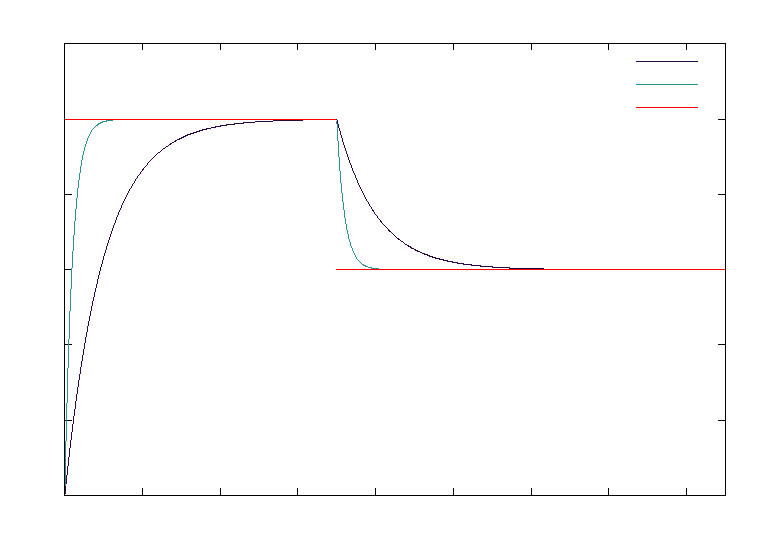
\includegraphics{plot/rc/double_rc}}%
    \gplfronttext
  \end{picture}%
\endgroup
}
				\caption{Andamento di $ v_1 $ e $ v_2 $ per $ \tau_1 = 0.01s $ e $ \tau_2 = 0.002s $}
			\end{figure}
		
			\paragraph{Osservazione}
			Ragionando intuitivamente sul grafico potremmo pensare che in realt\'a questo sistema non \textit{raggiunge} qualunque coppia di stati noi desideriamo $ (x_1, x_2) $ con $ x_1 \neq x_2 $, perch\'e la tensione sui condensatori va sempre a stabilizzarsi asintoticamente alla tensione imposta dal generatore. In realt\'a per \textit{raggiungere} uno stato, basta che lo stato del sistema assuma quel valore in un certo istante di tempo.
			
			Se lo stato assume un valore e lo mantiene, allora si tratta di un punto di equilibrio. Infatti \'e facile intuire che i punti di equilibrio di questo sistema sono caratterizzati dalla relazione $ u = x_1 = x_2 $. Verifichiamolo:
			\[ (\tilde x, \tilde u)\ \text{\'e punto di equilibrio}\ \Leftrightarrow A\tilde x + B \tilde u = 0 \]
			\[
				-\begin{bmatrix}
					-\alpha_1 & 0\\
					0 & -\alpha_2
				\end{bmatrix}
				\begin{bmatrix}
					\tilde x_1\\
					\tilde x_2
				\end{bmatrix} =
				\begin{bmatrix}
					\alpha_1\\
					\alpha_2
				\end{bmatrix} \tilde u \qquad\Rightarrow
				\begin{bmatrix}
					\alpha_1 \tilde x_1\\
					\alpha_2 \tilde x_2
				\end{bmatrix} =
				\begin{bmatrix}
					\alpha_1 \tilde u\\
					\alpha_2 \tilde u
				\end{bmatrix} \qquad\Rightarrow
				\begin{cases}
					\tilde x_1 &= \tilde u\\
					\tilde x_2 &= \tilde u
				\end{cases}
			\]
			Quindi i punti di equilibrio sono $ A = (\tilde x, \tilde u) = \left[ (\beta, \beta), \beta \right] $
		\end{Exercise}
	
		\begin{Exercise}[title={Studiare la controllabilit\'a di due vasche in parallelo}, difficulty=2]
			Consideriamo l'esempio del sistema non lineare delle vasche:
			\[ \dot h = \dfrac{1}{S}u - \dfrac{E}{S}\sqrt{2gh} \]
			Linearizzato attorno al punto di equilibrio $ (\tilde h, \tilde u) $:
			\[ \dot{\delta h} = -\alpha \delta h + \beta \delta u \]
			\[ \delta h = h - \tilde h \qquad \delta u = u - \tilde u \]
			
			Se abbiamo due vasche in parallelo:
			\[
				\begin{cases}
					\dot{\delta h_1} &= -\alpha_1 \delta h_1 + \dfrac{\beta_1}{2} \delta u\\
					\dot{\delta h_2} &= -\alpha_2 \delta h_2 + \dfrac{\beta_2}{2} \delta u
				\end{cases}
			\]
			\[
				\begin{bmatrix}
					-\alpha_1 & 0\\
					0 & -\alpha_2
				\end{bmatrix} \qquad
				\begin{bmatrix}
					\dfrac{\beta_1}{2}\\
					\dfrac{\beta_2}{2}\\
				\end{bmatrix}
			\]
			\[
				P=
				\begin{bmatrix}
					\dfrac{\beta_1}{2} & | & -\dfrac{\alpha_1 \beta_1}{2}\\
					\dfrac{\beta_2}{2} & | & -\dfrac{\alpha_2 \beta_2}{2}
				\end{bmatrix}\qquad
				\det(P) = -\dfrac{\alpha_2 \beta_1 \beta_2}{4} + \dfrac{\alpha_1 \beta_1 \beta_2}{4} = \dfrac{\beta_1 \beta_2}{4} \left( \alpha_1 - \alpha_2 \right)
			\]
			\[ \alpha_1, \alpha_2, \beta_1, \beta_2 \neq 0 \]
			
			Il sistema linearizzato \'e completamente controllabile se e solo se $ \alpha_1 \neq \alpha_2 $.
		\end{Exercise}
	
	\subsection{Nota sul prodotto di matrici}
		Date due matrici $ R $ e $ C $ compatibili per il prodotto righe per colonne $ RC $. Dividiamo le matrici in blocchi: $ R_1 $ e $ R_2 $ per $ R $; $ C_1 $ e $ C_2 $ per $ C $
		\[
			\begin{bmatrix}
				R_1\\
				R_2
			\end{bmatrix}
			\begin{bmatrix}
				C_1 & C_2
			\end{bmatrix} =
			\begin{bmatrix}
				R_1 C_1 & R_1 C_2\\
				R_2 C_2 & R_2 C_2
			\end{bmatrix}
		\]
		\[
			\begin{bmatrix}
				R_1\\
				R_2
			\end{bmatrix} M
			\begin{bmatrix}
				C_1 & C_2
			\end{bmatrix} =
			\begin{bmatrix}
				R_1\\
				R_2
			\end{bmatrix}
			\begin{bmatrix}
				M C_1 & M C_2
			\end{bmatrix} =	
			\begin{bmatrix}
				R_1 M C_1 & R_1 M C_2\\
				R_2 M C_2 & R_2 M C_2
			\end{bmatrix}
		\]
		oppure
		\[
			\begin{bmatrix}
				R_1\\
				R_2
			\end{bmatrix} M
			\begin{bmatrix}
				C_1 & C_2
			\end{bmatrix} =
			\begin{bmatrix}
				M R_1\\
				M R_2
			\end{bmatrix}
			\begin{bmatrix}
				C_1 & C_2
			\end{bmatrix} =	
			\begin{bmatrix}
				R_1 M C_1 & R_1 M C_2\\
				R_2 M C_2 & R_2 M C_2
			\end{bmatrix}
		\]
		
	\subsection{Decomposizione canonica di raggiungibilit\'a}		
		Definiamo $ X_{NR} \triangleq X_R^{\perp} $, cio\'e $ X_{NR} $ \'e complemento ortogonale di $ X_R $: se $ \hat x \in X_R $ e $ \tilde x \in X_{NR} $, allora $ \hat x \cdot \tilde x = 0 $.\\
		Poich\'e il vettore nullo \'e ortogonale a qualunque vettore, esso \'e contenuto sia in $ X_R $ che in $ X_{NR} $.
		\newline
		
		Per costruzione $ dim\left( X_R \right) = n_x - n_R $. Quindi se $ X_R = \R^{n_x} $ allora $ X_{NR} = \{0\} $. Viceversa se $ X_{NR} = \R^{n_x} $, allora $ X_R = \{0\} $
		\newline
		
		$ X_{NR} $ non va confuso con l'insieme di tutti e soli gli stati non raggiungibili, ma \'e un sottospazio che definiamo artificiosamente.
		\newline
		
		Se uno stato non \'e raggiungibile non significa che non potr\'a mai essere raggiunto, ma che non pu\'o essere raggiunto partendo dall'origine. Se lo stato parte fuori da $ X_R $, potr\'a raggiungere stati che non appartengono a $ X_R $.
		\newline
		
		Prendiamo per esempio il caso di $ n_x = 3 $: se $ X_R $ \'e una retta, $ X_{NR} $ \'e il piano perpendicolare; viceversa se $ X_R $ \'e un piano, $ X_{NR} $ \'e la retta perpendicolare;
		\newline
		
		Prendiamo:
		\begin{itemize}
			\item
				una base di $ X_R $ costituita da $ n_R = dim(X_R) $ elementi;
			\item
				una matrice $ T_1 \in \R^{n_x \times n_R} $, le cui colonne sono base di $ X_R $;
			\item
				una matrice $ T_2 \in \R^{n_x \times (n_x - n_R)} $, le cui colonne sono una base di $ X_{NR} $.
		\end{itemize}
	
		Costruiamo una nuova matrice quadrata:
		\[ T = \left[ T_1 | T_2 \right] \in \R^{n_x \times n_x} \]
		Tutte le colonne di $ T $ sono linearmente indipendenti perch\'e le colonne di $ T_1 $ sono ortogonali alle colonne di $ T_2 $. Quindi $ T $ \'e invertibile.
		
		Suddividiamo $ T^{-1} $ in due sottoblocchi:
		\[
			T^{-1} =
			\begin{bmatrix}
				H_1\\
				H_2
			\end{bmatrix}
		\]
		Per definizione di matrice invertibile $ T T^{-1} = T^{-1} T = I $:
		\[
			T^{-1} T =
			\begin{bmatrix}
				H_1\\
				H_2
			\end{bmatrix}
			\begin{bmatrix}
				T_1 & T_2
			\end{bmatrix} =
			\begin{bmatrix}
				H_1 T_1 & H_1 T_2\\
				H_2 T_1 & H_2 T_2 
			\end{bmatrix} = I =
			\begin{bmatrix}
				I & 0\\
				0 & I
			\end{bmatrix}
		\]
		\[ \Rightarrow H_1 T_2 = [0] \qquad H_2 T_1 = [0] \]
		In particolare dal secondo prodotto otteniamo che le righe di $ H_2 $ sono ortogonali alle colonne di $ T_1 $, quindi le righe di $ H_2 $ sono ortogonali alla base di $ X_R $: $ H_2 \perp X_R $.
		\newline
		
		Effettuiamo il cambio di base attraverso la matrice $ T $:
		\[ x = Tz \quad\Rightarrow\quad \dot z = T^{-1}AT z + T^{-1} B u = \tilde A z + \tilde B u \]
		\[
			\tilde A =
			\begin{bmatrix}
				H_1\\
				H_2
			\end{bmatrix} A
			\begin{bmatrix}
				T_1 & T_2
			\end{bmatrix} =
			\begin{bmatrix}
				H_1 A T_1 & H_1 A T_2\\
				H_2 A T_1 & H_2 A T_2
			\end{bmatrix}
		\]
		Concentriamoci sulla (2-1)-esima sottomatrice $ H_2 A T_1 $: $ T_1 $ \'e una base di $ X_R $ e $ X_R $ \'e invariante rispetto ad A $ \Rightarrow AT_1 \in X_R \Rightarrow H_2 \perp AT_1 $ perch\'e $ H_2 \perp X_R \Rightarrow H_2 A T_1 = 0 $
		\[
			\Rightarrow \tilde A = \begin{bmatrix}
				\tilde A_{11} & \tilde A_{12}\\
				0 & \tilde A_{22}
			\end{bmatrix}
		\]
		
		Invece per $ \tilde B $:
		\[
			\tilde B=
			\begin{bmatrix}
				H_1\\
				H_2
			\end{bmatrix} B =
			\begin{bmatrix}
				H_1 B\\
				H_2 B
			\end{bmatrix}
		\]
		Per il teorema di Kalmann le colonne di $ B $ appartengono a $ X_R $ quindi $ H_2 \perp B $
		\[
			\Rightarrow \tilde B =
			\begin{bmatrix}
				H_1 B\\
				0
			\end{bmatrix} =
			\begin{bmatrix}
					\tilde B_1\\
					0
			\end{bmatrix}
		\]
		
		Riscriviamo il sistema che abbiamo ottenuto:
		\[
			\begin{bmatrix}
				\dot z_R\\
				\dot z_{NR}
			\end{bmatrix}
			\begin{matrix}
				\left. \right\rbrace n_R \phantom{R}\\
				\left. \right\rbrace n_{NR}
			\end{matrix} =
			\begin{bmatrix}
				\tilde A_{11} & \tilde A_{12}\\
				0 & \tilde A_{22}
			\end{bmatrix} z +
			\begin{bmatrix}
				\tilde B_1\\
				0
			\end{bmatrix} u
		\]
		Con questo cambiamento di base abbiamo ottenuto che le prime $ n_R $ componenti sono raggiungibili, le ultime $ n_{NR} $ non sono raggiungibili. Abbiamo messo in ordine la struttura della matrice. Strutturalmente $ z_{NR} $ \'e non raggiungibile perch\'e \'e indipendente dal controllo, invece $ z_R $ \'e completamente raggiungibile.
		
		\begin{Exercise}[title={Calcolo di $ X_R $ e decomposizione di raggiungibilit\'a}, difficulty=1]
			Dato il sistema:
			\[
				\dot x =
				\begin{bmatrix}
					-1 & 0\\
					0 & -1
				\end{bmatrix} x +
				\begin{bmatrix}
					1\\
					1
				\end{bmatrix} u =
				\begin{cases}
					\dot x_1 &= -x_1+u\\
					\dot x_2 &= -x_2+u
				\end{cases}
			\]
			\[
				P = \left[ B | AB \right] =
				\begin{bmatrix}
					1 & | & -1\\
					1 & | & -1
				\end{bmatrix}
			\]
			\[ det(P) = 0 \quad\Rightarrow\quad rank(P) = dim(X_R) = 1 \]
			Infatti si pu\'o osservare che si tratta di due sistemi indipendenti tra loro, ma pilotati dallo stesso controllo: se partono dallo stesso stato si muovono in sincronia.
			\[
				X_R = \begin{bmatrix}
					\alpha\\
					\alpha
				\end{bmatrix}
			\]
			\'E l'insieme degli stati per cui $ x_1 = x_2 $.
			\newline
			
			Prendiamo la matrice $ T_1 $ la cui colonna sia base di $ X_R $ e la matrice $ T_2 $ la cui colonna sia base di $ X_{NR} $ (cio\'e un vettore ortogonale a $ T_1 $):
			\[
				T_1=
				\begin{bmatrix}
					1\\
					1
				\end{bmatrix} \qquad
				T_2=
				\begin{bmatrix}
					1\\
					-1
				\end{bmatrix}
			\]
			Quindi effettuiamo il cambio di base attraverso la matrice $ T $:
			\[
				T =
				\begin{bmatrix}
					T_1 & | & T_2	
				\end{bmatrix} =
				\begin{bmatrix}
					1 & 1\\
					1 & -1
				\end{bmatrix}\qquad
				T^{-1} =
				\begin{bmatrix}
					1 & 1\\
					1 & -1
				\end{bmatrix}^{-1} = -\dfrac{1}{2}
				\begin{bmatrix}
					-1 & -1\\
					-1 & 1
				\end{bmatrix}= \dfrac{1}{2}
				\begin{bmatrix}
					1 & 1\\
					1 & -1
				\end{bmatrix}
			\]
			\[ x = Tz \quad\Rightarrow\quad \dot z = \tilde A + \tilde B u \]
			\begin{align*}
				\tilde A &= T^{-1}AT = \dfrac{1}{2}
				\begin{bmatrix}
					1 & 1\\
					1 & -1
				\end{bmatrix}
				\begin{bmatrix}
					-1 & 0\\
					0 & -1
				\end{bmatrix}
				\begin{bmatrix}
					1 & 1\\
					1 & -1
				\end{bmatrix} =
				\begin{bmatrix}
					-1 & 0\\
					0 & -1
				\end{bmatrix}\\
				\tilde B &= T^{-1}B = \dfrac{1}{2}
				\begin{bmatrix}
					1 & 1\\
					1 & -1
				\end{bmatrix}
				\begin{bmatrix}
					1\\
					1
				\end{bmatrix} = \dfrac{1}{2}
				\begin{bmatrix}
					2\\
					0
				\end{bmatrix}=
				\begin{bmatrix}
					1\\
					0
				\end{bmatrix}
			\end{align*}
			\[
				\Rightarrow \dot z=
				\begin{bmatrix}
					-1 & 0\\
					0 & -1
				\end{bmatrix} z +
				\begin{bmatrix}
					1\\
					0
				\end{bmatrix} u
			\]
			Applichiamo il teorema di Kalmann e calcoliamo $ \tilde P $:
			\[
				\tilde P =
				\begin{bmatrix}
					1 & | & \dots\\
					0 & | & \dots
				\end{bmatrix}
			\]
			Poich\'e $ n_R = 1 $ e $ X_R $ \'e invariante al cambiamento di base, posso fermarmi alla prima colonna di $ \tilde P $:
			\[
				Z_R = \alpha
				\begin{bmatrix}
					1\\
					0
				\end{bmatrix}
			\]
		\end{Exercise}
	
	\subsection{Polinomio caratteristico di controllabilit\'a}
		Dato il sistema su cui \'e stata effettuata una decomposizione di raggiungibilit\'a attraverso la matrice $ T $:
		\[ \dot x = Ax+Bu \quad\xrightarrow{x=Tz}\quad \dot z = \tilde Az + \tilde Bu \]
		Consideriamo l'evoluzione forzata dello stato:
		\[ \Lapl{x_f(t) = \int_{0^-}^{t}e^{A(t-\tau)Bu(\tau)d\tau}}{X_f(s) = (sI-A)^{-1} B U(s)} \]
		Per la linearit\'a della trasformata di Laplace:
		\[ \Lapl{z(t) = T^{-1} x(t)}{Z(s) = T^{-1} X(s)} \]
		\begin{align*}
			\Rightarrow Z_f(s) &= (sI-\tilde A)^{-1} \tilde B U(s) =\\
			&= (s T^{-1} I T - T^{-1} A T )^{-1} T^{-1} B U(s) =\\
			&= (T^{-1} sI T - T^{-1} A T )^{-1} T^{-1} B U(s) =\\
			&= (T^{-1} (sI-A) T)^{-1} T^{-1} B U(s) =\footnotemark\\
			&= (T^{-1} (sI-A)^{-1} T) T^{-1} B U(s) = T^{-1} X_f(s)
		\end{align*}
		\footnotetext{$ (AB)^{-1} = B^{-1}A^{-1} $}
		
		\setword{Quindi studiare $ (sI-A)^{-1} B U(s) $ o $ (sI-\tilde A)^{-1} \tilde B U(s) $ \'e equivalente a meno di un $ T^{-1}. $}{sentece:calcolo-autovalori}
		\newline
		
		Il polinomio caratteristico (e anche il polinomio minimo) \'e invariante al cambio di base:
		\[ \phi(s) = \tilde \phi(s) \qquad \big(  m(s) = \tilde m(s) \big) \]
		\begin{align*}
			\tilde \phi(s) &= det(sI-\tilde A) = det(s T^{-1} I T - T^{-1} A T) =\\
			&= det(T^{-1} (sI-A) T) = det(T^{-1}) det(sI-A) det(T) =\footnotemark det(sI-A) 
		\end{align*}
		\footnotetext{$ det(T) \cdot det(T^{-1}) = 1 $}
		
		Calcoliamo gli autovalori nella nuova base:
		\begin{align*}
			\phi(s) &= \tilde \phi(s) = det(sI-\tilde A) =\\
			&= det\left\lbrace s
			\begin{bmatrix}
				I_{n_R} & 0\\
				0 & I_{n_{NR}}
			\end{bmatrix} -
			\begin{bmatrix}
				\tilde A_{11} & \tilde A_{12}\\
				0 & \tilde A_{22}
			\end{bmatrix} \right\rbrace =\\
			&=
			\begin{bmatrix}
				(sI-\tilde A_{11}) & -\tilde A_{12}\\
				0 & (sI-\tilde A_{22})
			\end{bmatrix} =\\
			&= \underbrace{det(sI-\tilde A_{11})}_{\phi_C(s)} \cdot \underbrace{det(sI-\tilde A_{22})}_{\phi_{NC}(s)}
		\end{align*}
		\begin{itemize}
			\item
				$ \phi_C(s) $ \'e il \textbf{polinomio caratteristico di controllabilit\'a}. Le radici di $ \phi_C(s) $ sono gli autovalori di $ \tilde A_{11} $, che \'e la parte controllabile del sistema, e sono detti \textbf{autovalori controllabili}.
			\item
				$ \phi_{NC}(s) $ \'e il \textbf{polinomio caratteristico di non controllabilit\'a}. Le radici di $ \phi_{NC}(s) $ sono gli autovalori di $ \tilde A_{11} $, che \'e la parte non controllabile del sistema, e sono detti \textbf{autovalori non controllabili}.
		\end{itemize}
	
	\subsubsection{Come calcolare gli autovalori controllabili}
		\begin{align*}
			(sI-\tilde A)^{-1} \tilde B &=
			\begin{bmatrix}
				(sI-\tilde A_{11}) & -\tilde A_{12}\\
				0 & (sI-\tilde A_{22})
			\end{bmatrix}^{-1}
			\begin{bmatrix}
				\tilde B_1\\
				0
			\end{bmatrix} =\\
			&= \begin{bmatrix}
				(sI-\tilde A_{11})^{-1} & M_{12}(s)\\
				0 & (sI-\tilde A_{22})^{-1}
			\end{bmatrix}
			\begin{bmatrix}
				\tilde B_1\\
				0
			\end{bmatrix} =\\
			&= \begin{bmatrix}
				(sI-\tilde A_{11})^{-1} \tilde B_1\\
				0
			\end{bmatrix}
		\end{align*}
		$ (sI-\tilde A)^{-1} \tilde B $ non ha informazioni su $ \tilde A_{22} $.
		
		\'E evidente che il polinomio caratteristico associato a $ (sI-\tilde A_{11}) \tilde B_1 $ equivale a quello di $ (sI - \tilde A)^{-1} \tilde B $, perch\'e le due matrici differiscono per un blocco di zeri (che non avendo un denominatore non influiscono sul polinomio caratteristico).\\
		Si pu\'o dimostrare che il polinomio caratteristico associato a $ (sI-\tilde A_{11})^{-1} \tilde B_1 $ coincide con $ \phi_C(s) = det(sI-\tilde A_{11}) $. Quindi per calcolare $ \phi_C(s) $ \'e sufficiente calcolare il polinomio caratteristico associato a $ (sI-\tilde A)^{-1} \tilde B $.
		
		Ma per \hyperref[sentece:calcolo-autovalori]{quanto gi\'a detto}, studiare $ (sI-A)^{-1} B $ equivale a studiare $ (sI-\tilde A)^{-1} \tilde B $ a meno di $ T^{-1} $. Quindi per calcolare $ \phi_C(s) $ basta calcolare il polinomio caratteristico associato a $ (sI-A)^{-1} B $.
\end{document}